\begin{frame}{Regularization}

    \centering
    \Huge{\textbf{Regularization}}

    \vfill

    \small{Slides from: \url{https://harvard-iacs.github.io/2019-CS109A/lectures/lecture8/presentation/Lecture8a_Regularization.pptx}}

\end{frame}

\begin{frame}{Regularization: An Overview}
    \begin{itemize}
        \item Regularization involves modifying the loss function $L$ to improve model generalization.
        \item A regularization term is added to penalize certain properties of the model parameters:
        \[
            L_{\text{reg}}(\beta) = L(\beta) + \lambda R(\beta)
        \]
        \item $\lambda$ is a scalar that controls the strength of the regularization.
        \item The function $R(\beta)$ encodes the properties to penalize (e.g., large coefficients).
        \item Minimizing $L_{\text{reg}}$ leads to model parameters with more desirable characteristics.
    \end{itemize}
\end{frame}


\begin{frame}[allowframebreaks]{LASSO Regression}
    \begin{itemize}
        \item LASSO discourages extreme values in model parameters by penalizing their magnitudes.
        \item We use MSE as the base loss function.
        \item The regularized loss function is:
        \[
            L_{\text{LASSO}}(\beta) = \frac{1}{n} \sum_{i=1}^{n} \left| y_i - \beta^\top x_i \right|^2 + \lambda \sum_{j=1}^{J} |\beta_j|
        \]
        \item The term \( \sum_{j=1}^{J} |\beta_j| \) is the \( \ell_1 \) norm of the vector \( \beta \):
        \[
            \sum_{j=1}^{J} |\beta_j| = \|\beta\|_1
        \]
    \end{itemize}
\end{frame}

\begin{frame}[allowframebreaks]{Ridge Regression}
    \begin{itemize}
        \item Regularization term penalizes the \textbf{squares} of the parameter magnitudes.
        \item The regularized loss function becomes:
        \[
            L_{\text{Ridge}}(\beta) = \frac{1}{n} \sum_{i=1}^{n} \left| y_i - \beta^\top x_i \right|^2 + \lambda \sum_{j=1}^{J} \beta_j^2
        \]
        \item Note that:
        \[
            \sum_{j=1}^{J} \beta_j^2 = \|\beta\|_2^2
        \]
        which is the square of the \( \ell_2 \)-norm of \( \beta \).
    \end{itemize}
\end{frame}


\begin{frame}{Choosing \( \lambda \)}
    \begin{itemize}
        \item In both ridge and LASSO regression, the larger the regularization parameter \( \lambda \), the more we penalize large values in \( \beta \).
        \item If \( \lambda \) is close to zero:
        \begin{itemize}
            \item The penalty is minimal.
            \item We recover the MSE, i.e., ridge and LASSO become ordinary regression.
        \end{itemize}
        \item If \( \lambda \) is sufficiently large:
        \begin{itemize}
            \item The MSE term becomes negligible.
            \item The regularization forces \( \beta_{\text{ridge}} \) and \( \beta_{\text{LASSO}} \) close to zero.
        \end{itemize}
        \item To avoid ad-hoc selection, \( \lambda \) should be chosen via cross-validation.
    \end{itemize}
\end{frame}


\begin{frame}{Ridge, LASSO - Computational Complexity}
    \begin{itemize}
        \item \textbf{Ridge Regression Solution:}
        \[
            \beta = (X^T X + \lambda I)^{-1} X^T Y
        \]
        
        \item \textbf{LASSO Regression:}
        \begin{itemize}
            \item No closed-form analytical solution.
            \item The \( L_1 \) norm is not differentiable at 0.
            \item We use the concept of \textit{subdifferential} or \textit{subgradient} to derive manageable expressions.

        \end{itemize}
    \end{itemize}
\end{frame}


\begin{frame}{Regularization Parameter with a Validation Set}
    The solution of the Ridge/Lasso regression involves three steps:
    \begin{itemize}
        \item Select \( \lambda \)
        \item Find the minimum of the ridge/Lasso regression loss function (using the ridge formula), and record the \textbf{MSE on the validation/test set}.
        \item Find the \( \lambda \) that gives the smallest \( \text{MSE} \)
    \end{itemize}
\end{frame}


\begin{frame}{The Geometry of Regularization (LASSO)}
    \begin{itemize}
        \item[] \[
        L_{\text{LASSO}}(\boldsymbol{\beta}) = \frac{1}{n} \sum_{i=1}^n \left| y_i - \boldsymbol{\beta}^T \mathbf{x} \right|^2 + \lambda \sum_{j=1}^J |\beta_j|
        \]
        \item[] \[
        \hat{\boldsymbol{\beta}}^{\text{LASSO}} = \arg\min L_{\text{LASSO}}(\boldsymbol{\beta})
        \]
    \end{itemize}

    \begin{figure}
        \centering
        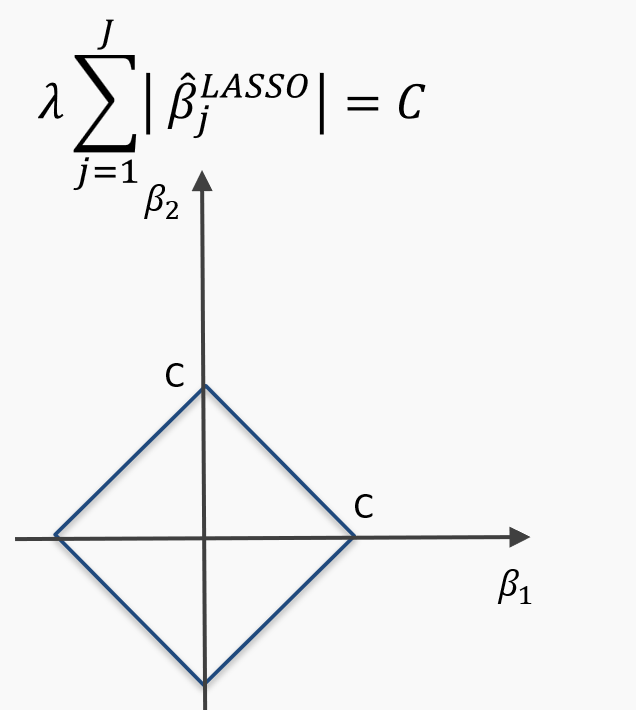
\includegraphics[width=0.35\textwidth]{images/linear-regression/linear-regression-22.png}
        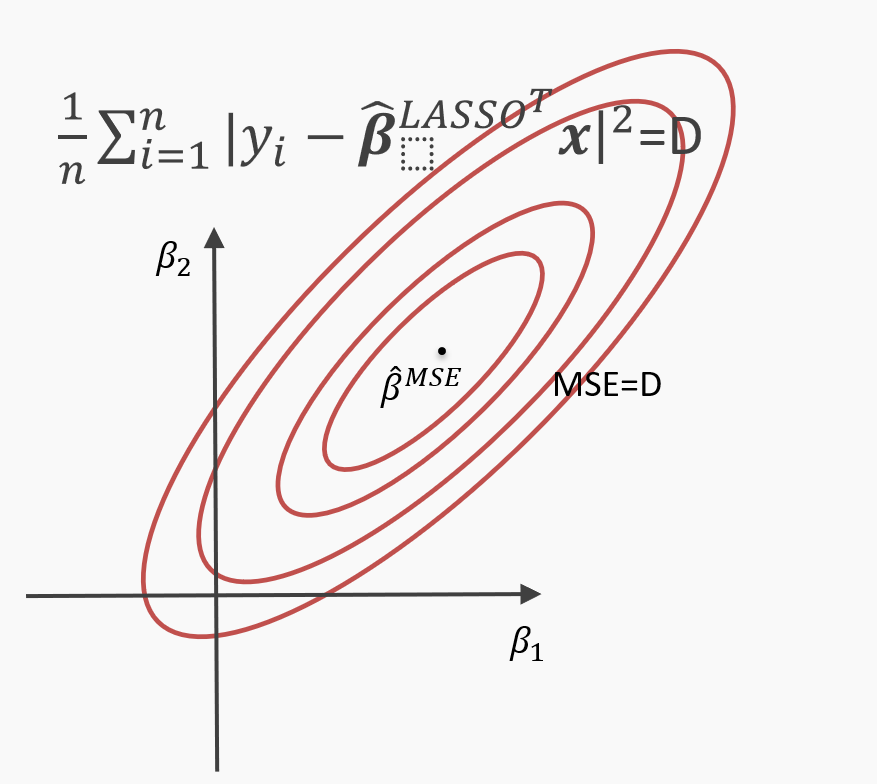
\includegraphics[width=0.35\textwidth]{images/linear-regression/linear-regression-23.png}
    \end{figure}
\end{frame}


\begin{frame}{The Geometry of Regularization (LASSO)}
    \begin{itemize}
        \item Regularized loss function:
        \[
            L_{\text{LASSO}}(\boldsymbol{\beta}) = \frac{1}{n} \sum_{i=1}^{n} \left| y_i - \boldsymbol{\beta}^T \mathbf{x} \right|^2 + \lambda \sum_{j=1}^{J} |\beta_j|
        \]
        \item LASSO solution:
        \[
            \hat{\boldsymbol{\beta}}^{\text{LASSO}} = \arg\min L_{\text{LASSO}}(\boldsymbol{\beta})
        \]
    \end{itemize}

    \vspace{1em}

    \begin{columns}
        \column{0.5\textwidth}
        \begin{itemize}
            \item $L_1 = \lambda \sum_{j=1}^{J} \left| \hat{\beta}_j^{\text{LASSO}} \right|$
        \end{itemize}
        \begin{center}
            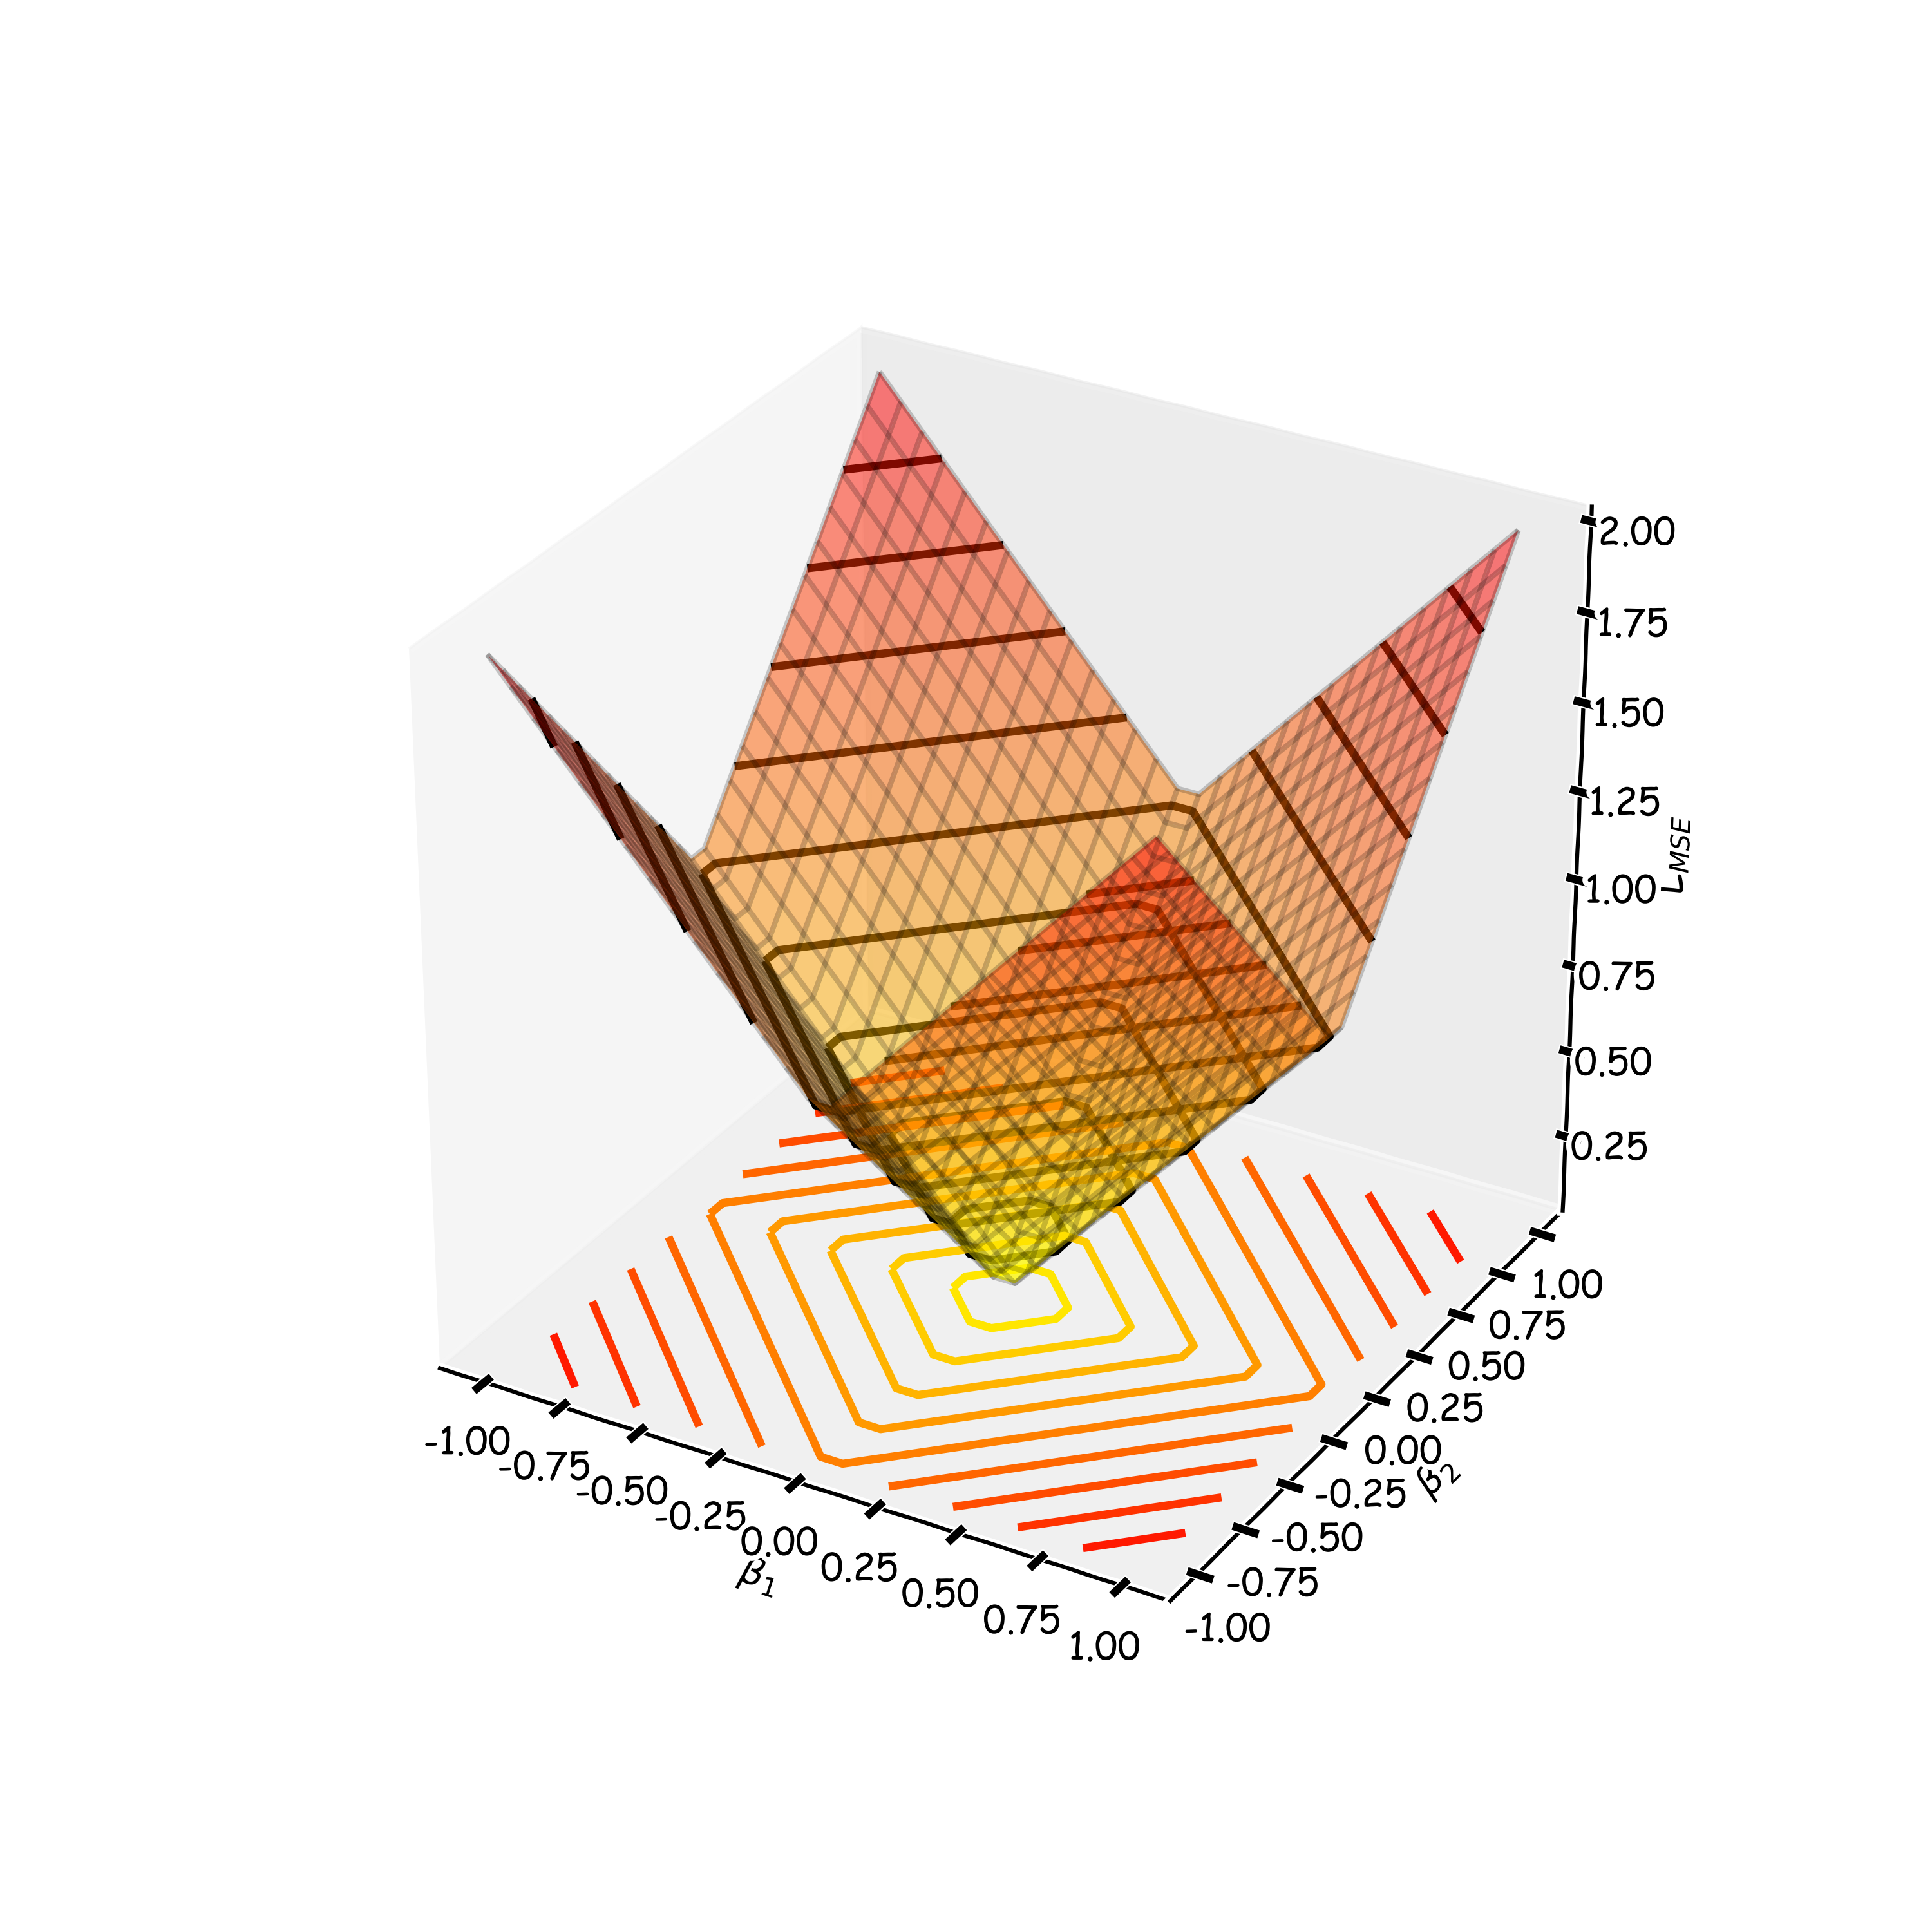
\includegraphics[height=3.5cm]{images/linear-regression/linear-regression-24.png}
        \end{center}

        \column{0.5\textwidth}
        \begin{itemize}
            \item $L_{\text{MSE}}(\boldsymbol{\beta}) = \frac{1}{n} \sum_{i=1}^{n} \left| y_i - \boldsymbol{\beta}^T \mathbf{x} \right|^2$
        \end{itemize}
        \begin{center}
            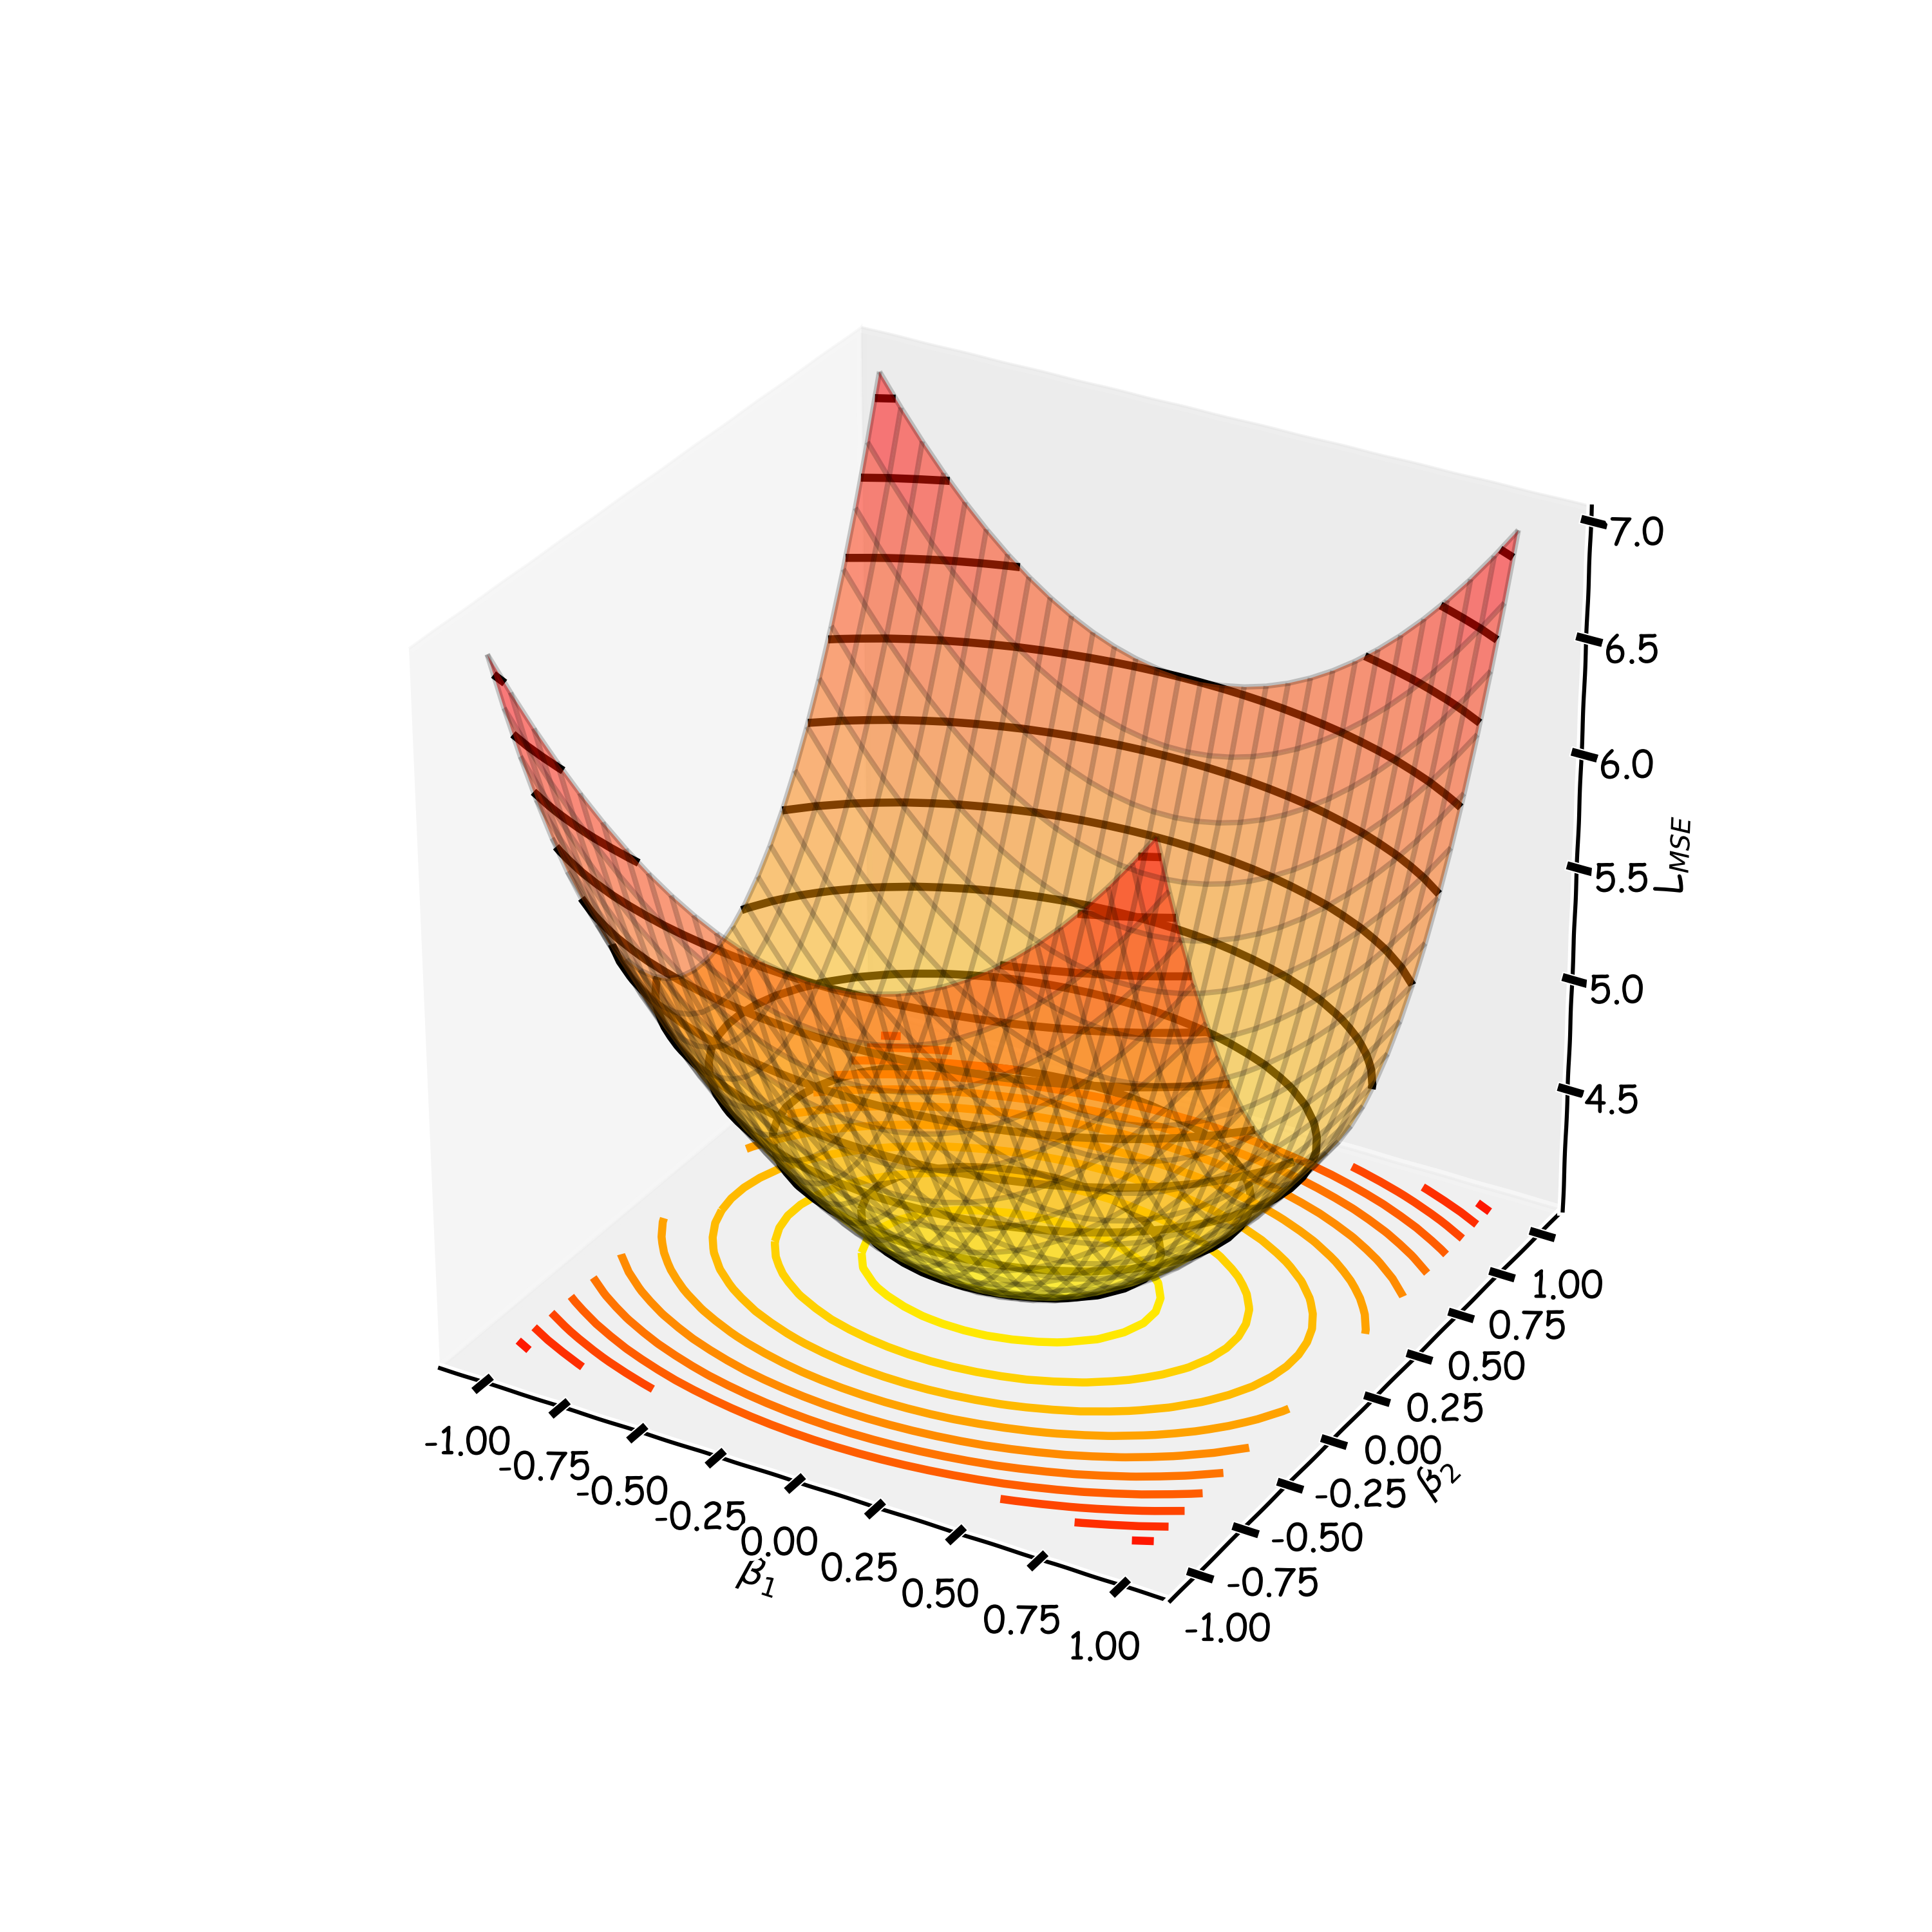
\includegraphics[height=3.5cm]{images/linear-regression/linear-regression-25.png}
        \end{center}
    \end{columns}
\end{frame}


\begin{frame}{LASSO visualized}
    \begin{columns}
        \column{0.5\textwidth}
        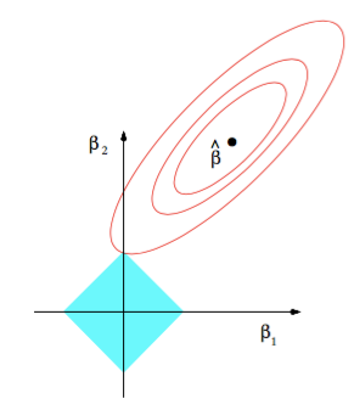
\includegraphics[height=4cm]{images/linear-regression/linear-regression-26.png}
        \begin{itemize}
            \item The LASSO estimator tends to zero out parameters.
            \item The OLS loss can easily intersect with the constraint on one of the axes.
        \end{itemize}

        \column{0.5\textwidth}
        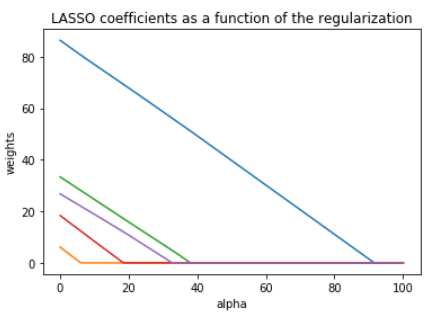
\includegraphics[height=4cm]{images/linear-regression/linear-regression-27.png}
        \begin{itemize}
            \item The values of the coefficients decrease as $\lambda$ increases.
            \item Coefficients are nullified quickly.
        \end{itemize}
    \end{columns}
\end{frame}


\begin{frame}{The Geometry of Regularization (Ridge)}

\begin{columns}
    \column{0.48\textwidth}
    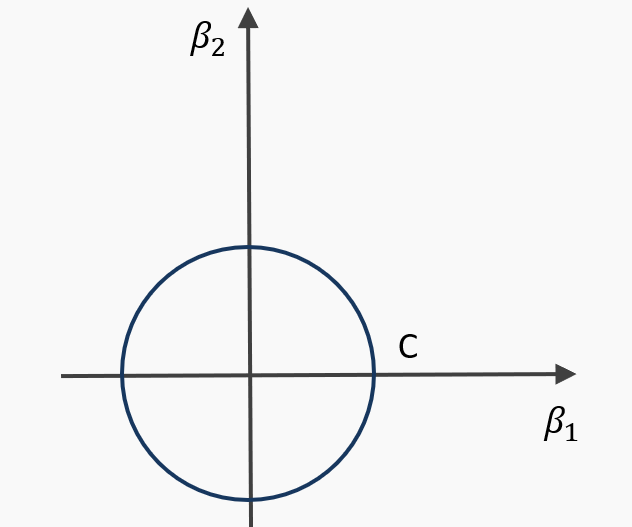
\includegraphics[width=\linewidth]{images/linear-regression/linear-regression-28.png}

    \begin{itemize}
        \item $L_{Ridge}(\boldsymbol{\beta}) = \frac{1}{n} \sum_{i=1}^n \left| y_i - \boldsymbol{\beta}^T \boldsymbol{x} \right|^2 + \lambda \sum_{j=1}^J (\beta_j)^2$
        \item $\hat{\boldsymbol{\beta}}^{Ridge} = \arg\min L_{Ridge}(\boldsymbol{\beta})$
        \item $\lambda \sum_{j=1}^J \left| \hat{\beta}_j^{Ridge} \right|^2 = C$
    \end{itemize}

    \column{0.48\textwidth}
    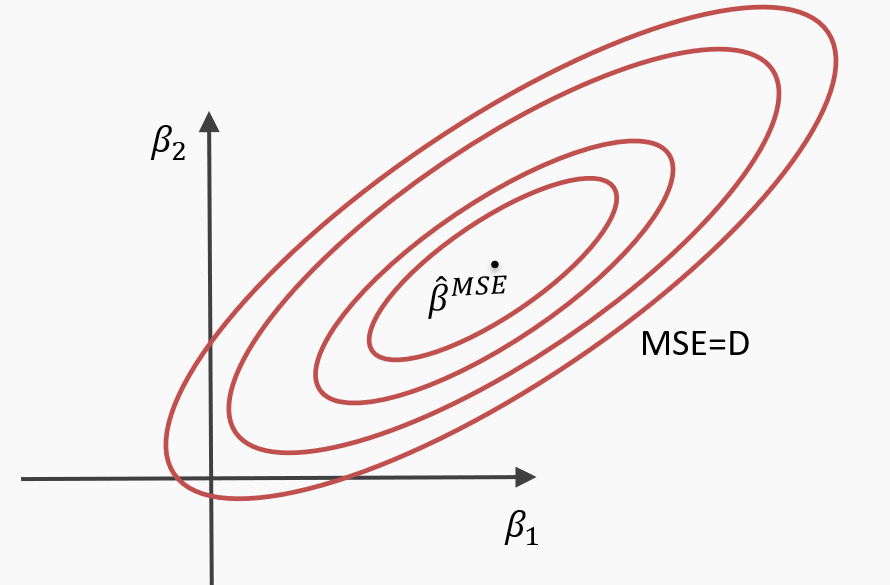
\includegraphics[width=\linewidth]{images/linear-regression/linear-regression-29.png}

    \begin{itemize}
        \item $\frac{1}{n} \sum_{i=1}^n \left| y_i - \hat{\boldsymbol{\beta}}^{Ridge\, T} \boldsymbol{x} \right|^2 = D$
        \item The ridge constraint forms a circle in 2D.
        \item The solution lies at the point where the MSE contour touches the constraint boundary.
    \end{itemize}

\end{columns}

\end{frame}


\begin{frame}{Ridge visualized}

\begin{columns}
    \column{0.48\textwidth}
    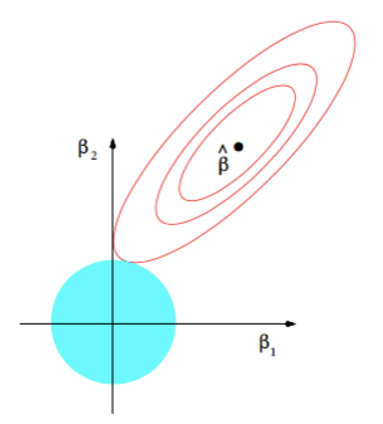
\includegraphics[width=\linewidth]{images/linear-regression/linear-regression-30.png}
    \begin{itemize}
        \item The ridge estimator is where the constraint and the loss intersect.
    \end{itemize}

    \column{0.48\textwidth}
    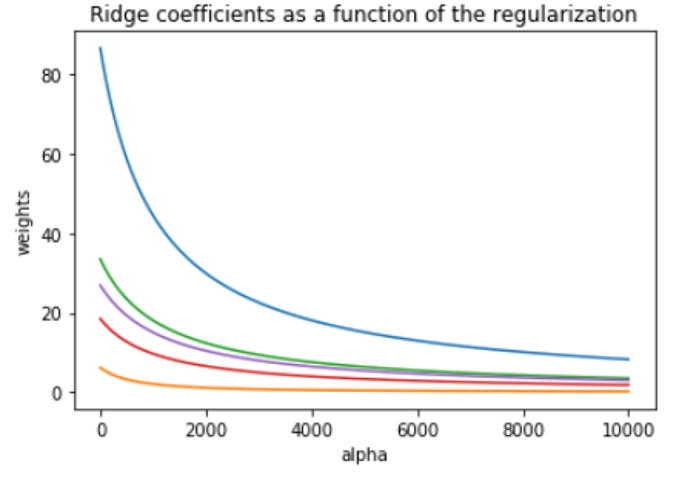
\includegraphics[width=\linewidth]{images/linear-regression/linear-regression-31.png}
    \begin{itemize}
        \item The values of the coefficients decrease as lambda increases, but they are not nullified.
    \end{itemize}
\end{columns}

\end{frame}


\begin{frame}{The Geometry of Regularization}

\begin{center}
    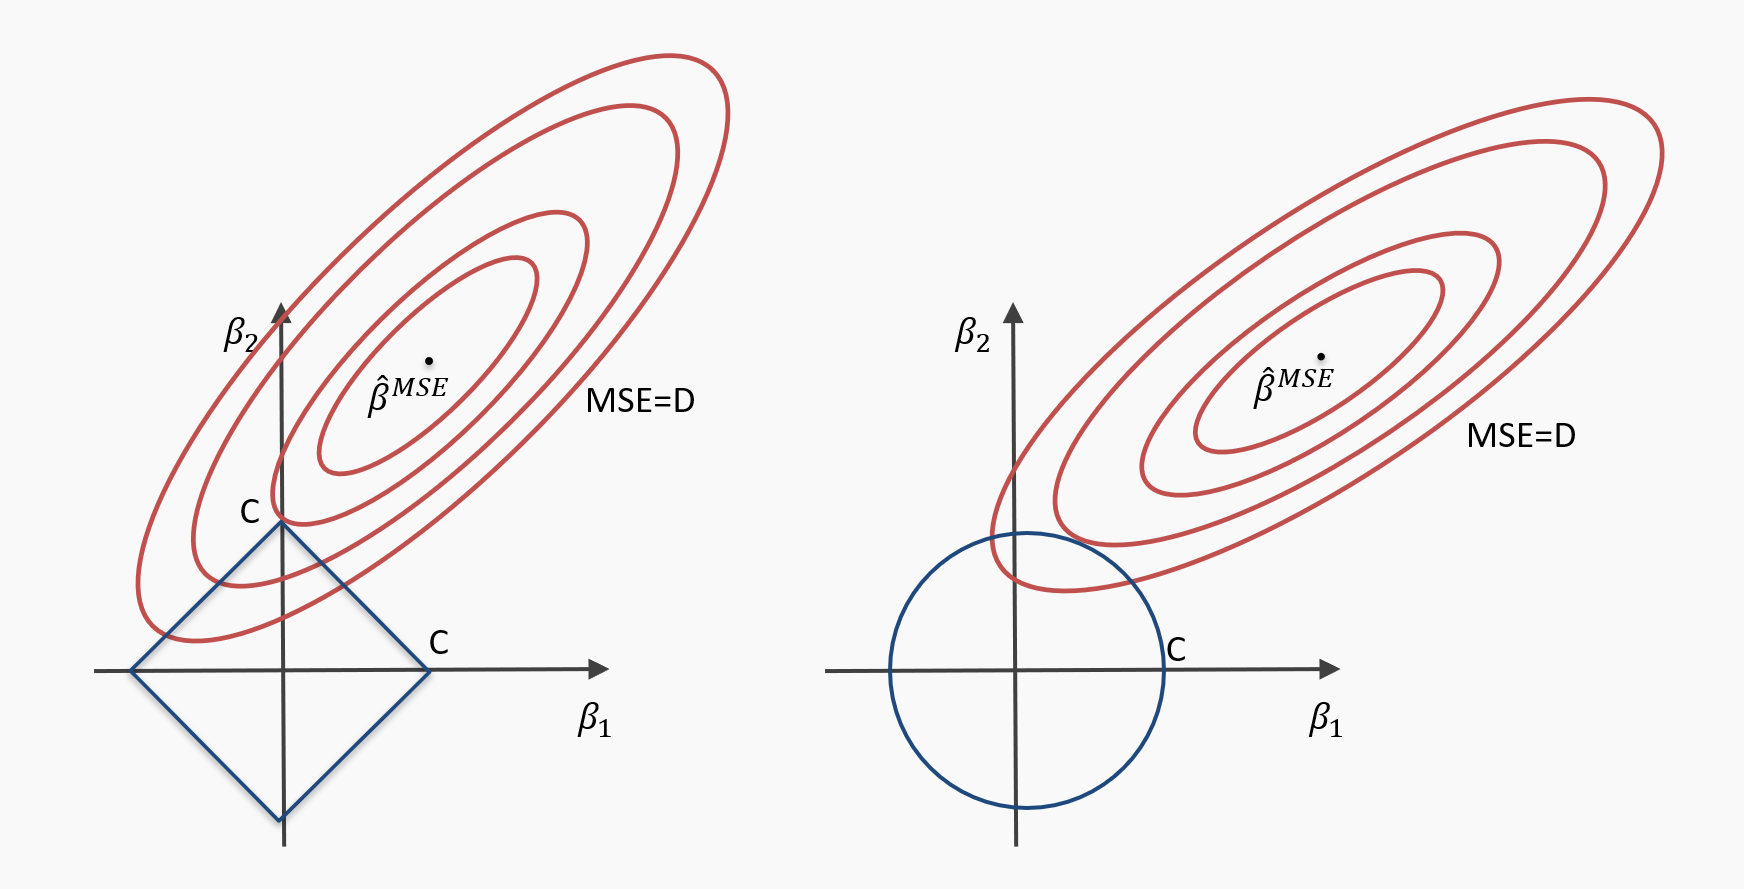
\includegraphics[width=0.9\linewidth]{images/linear-regression/linear-regression-32.png}
\end{center}

\end{frame}


\begin{frame}{Ridge regularization with only \textbf{validation}: step by step}
\begin{enumerate}
  \item Split data into $\{\{X, Y\}_{\text{train}}, \{X, Y\}_{\text{validation}}, \{X, Y\}_{\text{test}}\}$
  
  \item For $\lambda$ in $\{\lambda_{\min}, \dots, \lambda_{\max}\}$:
  \begin{enumerate}
    \item Determine the $\beta$ that minimizes the $L_{\text{ridge}}$:
    \[
    \hat{\beta}_{\text{Ridge}}(\lambda) = (X^T X + \lambda I)^{-1} X^T Y, \quad \text{using the train data}
    \]
    \item Record $L_{\text{MSE}}(\lambda)$ using validation data.
  \end{enumerate}
  
  \item Select the $\lambda$ that minimizes the loss on the validation data:
  \[
  \lambda_{\text{ridge}} = \arg\min_{\lambda} L_{\text{MSE}}(\lambda)
  \]
  
  \item Refit the model using both \textbf{train and validation} data:
  \[
  \{X, Y\}_{\text{train}}, \{X, Y\}_{\text{validation}} \Rightarrow \hat{\beta}_{\text{ridge}}(\lambda_{\text{ridge}})
  \]
  
  \item Report MSE or $R^2$ on $\{X, Y\}_{\text{test}}$ given the $\hat{\beta}_{\text{ridge}}(\lambda_{\text{ridge}})$
\end{enumerate}
\end{frame}


\begin{frame}{Lasso regularization with \textbf{validation only}: step by step}
\begin{enumerate}
    \item Split data into $\{ \{X, Y\}_{\text{train}}, \{X, Y\}_{\text{validation}}, \{X, Y\}_{\text{test}} \}$
    \item For $\lambda$ in $\{\lambda_{\min}, \dots, \lambda_{\max}\}$:
    \begin{enumerate}
        \item Determine the $\beta$ that minimizes the $L_{\text{lasso}}$,
        \[
        \hat{\beta}_{\text{lasso}}(\lambda),
        \]
        using the train data. \textbf{This is done using a solver}.
        \item Record $L_{\text{MSE}}(\lambda)$ using validation data.
    \end{enumerate}
    \item Select the $\lambda$ that minimizes the loss on the validation data:
    \[
    \lambda_{\text{lasso}} = \arg\min_{\lambda} L_{\text{MSE}}(\lambda)
    \]
    \item Refit the model using both \textbf{train} and \textbf{validation} data:
    \[
    \{X, Y\}_{\text{train}}, \{X, Y\}_{\text{validation}} \Rightarrow \hat{\beta}_{\text{lasso}}(\lambda_{\text{lasso}})
    \]
    \item Report MSE or $R^2$ on $\{X, Y\}_{\text{test}}$ given the $\hat{\beta}_{\text{lasso}}(\lambda_{\text{lasso}})$
\end{enumerate}
\end{frame}


\begin{frame}{Ridge regularization with \textbf{validation only}: step by step}
\centering
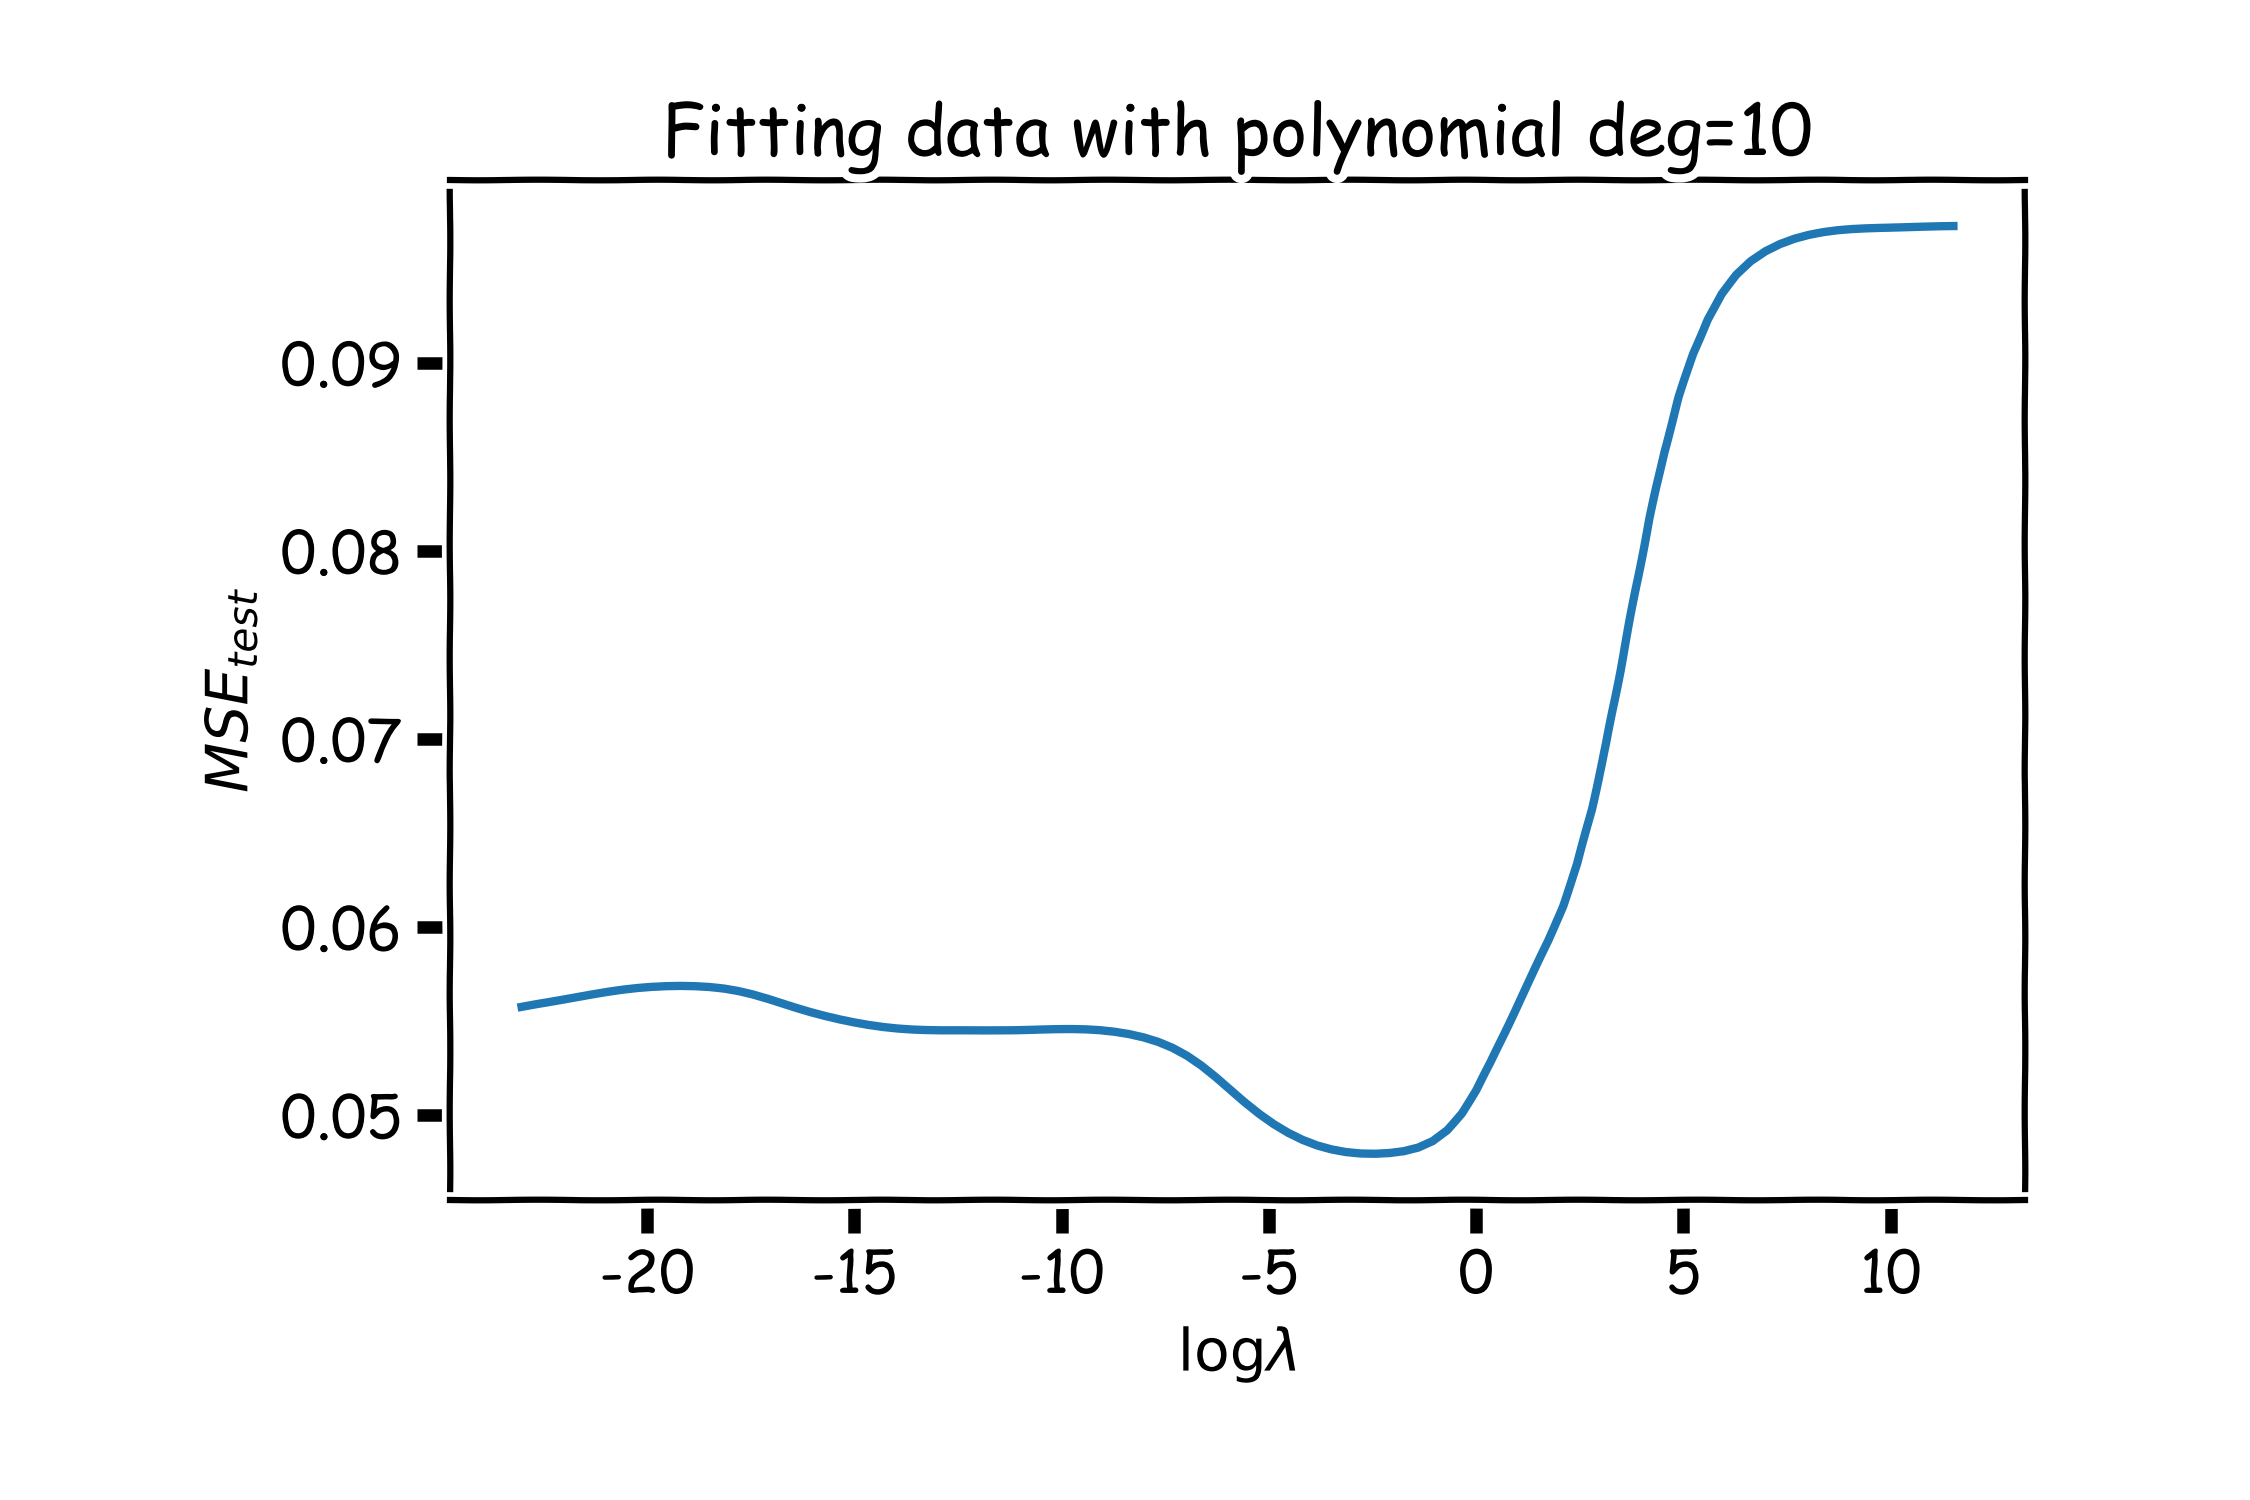
\includegraphics[width=0.85\linewidth]{images/linear-regression/linear-regression-33.png}

\end{frame}


\begin{frame}[allowframebreaks]{Ridge regularization with \textbf{CV}: step by step}
\begin{enumerate}
    \item Remove $\{X, Y\}_{\text{test}}$ from data.
    \item Split the rest of the data into $K$ folds:  
    $\left\{\{X, Y\}_{\text{train}}^{-k}, \{X, Y\}_{\text{val}}^k\right\}$
    
    \item For $k \in \{1, \dots, K\}$:
    \begin{enumerate}
        \item For $\lambda \in \{\lambda_0, \dots, \lambda_n\}$:
        \begin{itemize}
            \item Determine the $\beta$ that minimizes the $L_{\text{ridge}}$:
            \[
            \hat{\beta}_{\text{ridge}}(\lambda, k) = (X^\top X + \lambda I)^{-1} X^\top Y
            \]
            using the training data $\{X, Y\}_{\text{train}}^k$.
            \item Record $L_{\text{MSE}}(\lambda, k)$ using the validation data $\{X, Y\}_{\text{val}}^k$.
        \end{itemize}
    \end{enumerate}
    At this point, we have a 2D matrix: rows correspond to different $k$, and columns to different $\lambda$ values.

    \item Average the $L_{\text{MSE}}(\lambda, k)$ for each $\lambda$:
    \[
    \bar{L}_{\text{MSE}}(\lambda) = \frac{1}{K} \sum_{k=1}^{K} L_{\text{MSE}}(\lambda, k)
    \]

    \item Find the $\lambda$ that minimizes $\bar{L}_{\text{MSE}}(\lambda)$:  
    $\lambda_{\text{ridge}} = \arg\min_\lambda \bar{L}_{\text{MSE}}(\lambda)$

    \item Refit the model using the full training data  
    $\left\{\{X, Y\}_{\text{train}}, \{X, Y\}_{\text{val}}\right\} \Rightarrow \hat{\beta}_{\text{ridge}}(\lambda_{\text{ridge}})$

    \item Report MSE or $R^2$ on $\{X, Y\}_{\text{test}}$ using $\hat{\beta}_{\text{ridge}}(\lambda_{\text{ridge}})$
\end{enumerate}
\end{frame}


\begin{frame}{Ridge regularization with \textbf{CV} only: step by step}
\begin{figure}
    \centering
    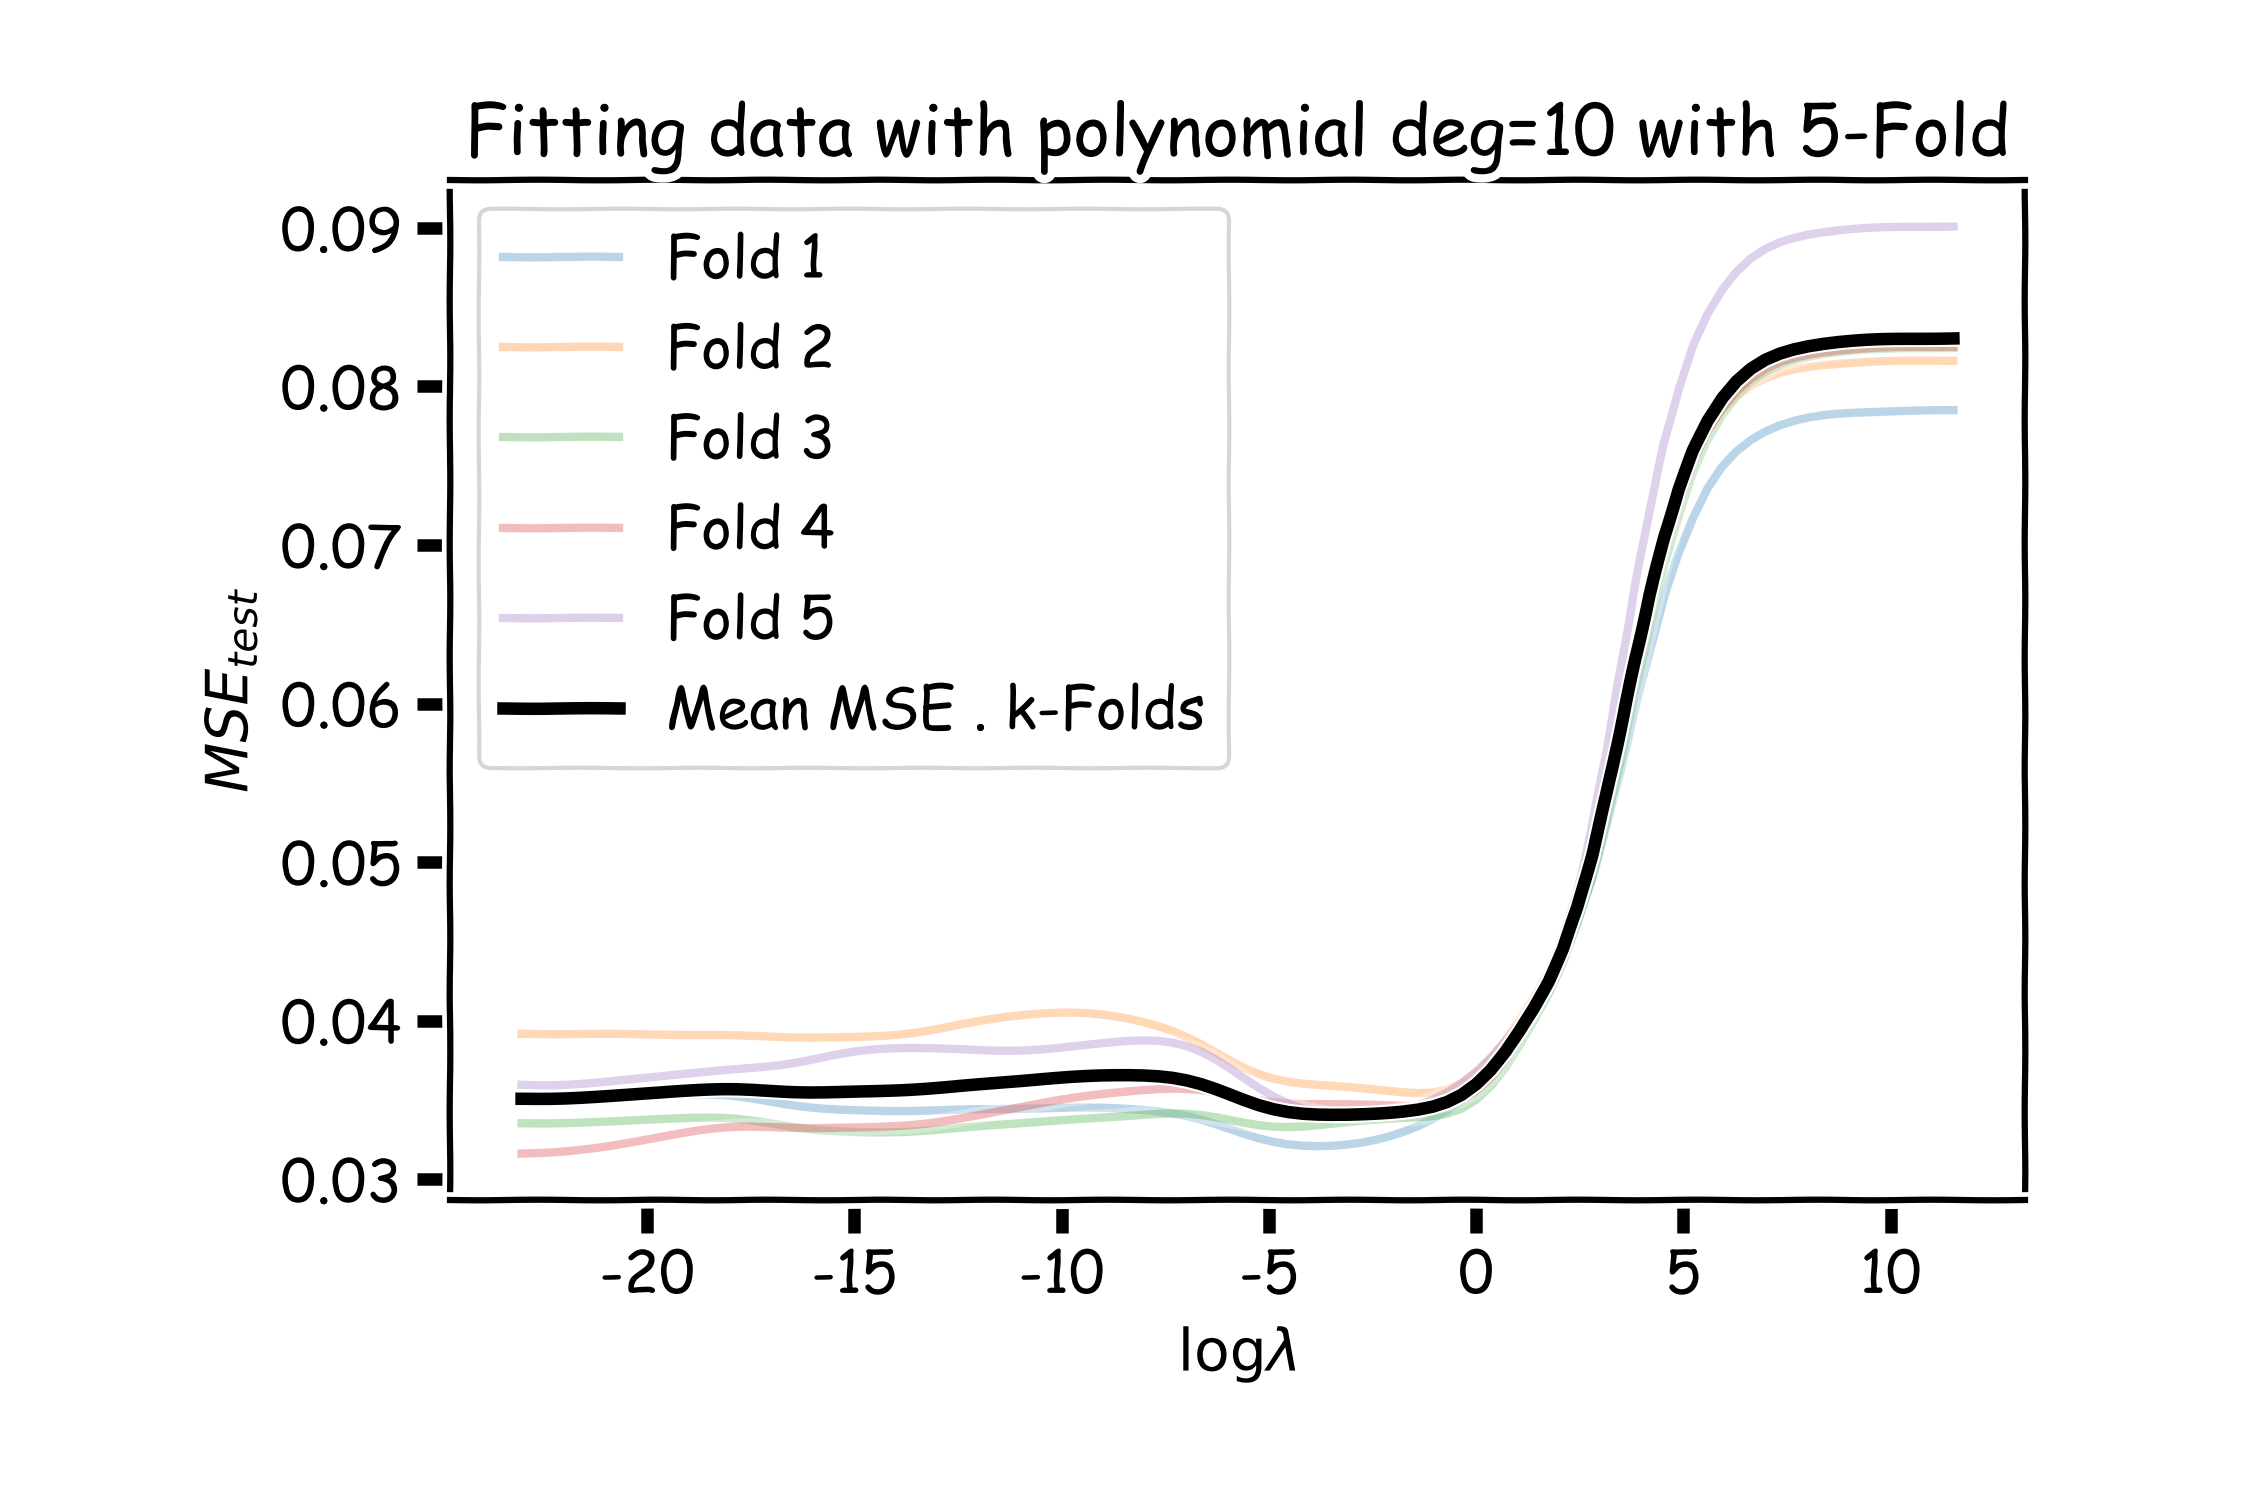
\includegraphics[width=0.9\textwidth]{images/linear-regression/linear-regression-34.png}
    \caption*{
        \small
        Validation error $MSE_{\text{val}}$ across $\lambda$ values (log scale) using 5-fold cross-validation. \\
        Each colored line corresponds to one fold. The thick black curve shows the mean validation error across all folds.
    }
\end{figure}
\end{frame}


\begin{frame}{Variable Selection as Regularization}

\begin{itemize}
    \item Since \textbf{LASSO} regression tends to produce zero estimates for a number of model parameters – we say that LASSO solutions are \textbf{sparse} – we consider LASSO to be a method for variable selection.
    
    \item Many prefer using LASSO for variable selection (as well as for suppressing extreme parameter values) rather than stepwise selection, as LASSO avoids the statistical problems that arise in stepwise selection.
    
    \item \textbf{Question:} What are the pros and cons of the two approaches?
\end{itemize}

\end{frame}
